\chapter{Optimizing Object Model and Calls}
\label{chp:ch5-object}

Python is an object oriented programing language.
It is a common practice for Python programmer to encode states using classes and encapsulate logic in methods in their programs.
As an implementation of the Python language, it is essential for us to ensure the performance of object operations and method calls in ZipPy.
In the previous chapters we discussed how we optimize arithmetics (Chapter~\ref{chp:ch3-zippy}) and accelerate iterators (Chapter~\ref{chp:ch4-peeling}).
In this chapter we explain how we implement object operations and calls in ZipPy.

\section{Object Model}
\label{sec:ch5-object-module}

\subsection{Python Object Data Representations}

In Python all data is an object.
CPython, the original implementation of Python, constructs every data type in Python as a heap allocated data structure.
Since it is written in C, CPython implements Python built-in data types using C struct and user defined types using hash maps.
This model results in expensive arithmetic operations due to frequent accesses and allocations of data structures in the heap.
Hash map based object model is also inefficient.
Although the cost of hash map operations is amortized for large data sets, the overhead of retrieving or updating a single map entry is still expensive.
In a hash map based object model, retrieving the value of an object field, or an object attribute in Python, is equivalent to reading the value of a map entry.
This operation involves a hashing calculation and a few steps of memory accesses before reaching the memory address that stores the target value.
On the other hand, in a traditional programming language like Java, an object field access, if optimized, is simply a single memory read.
In summary, object model inefficiency is the main impediment to the performance of popular dynamic languages like Python.

\subsubsection{Jython's Object Model Design}

Existing JVM based Python implementations like Jython, however, replicate the same object model design we saw in CPython.
The main approach they are took is porting the existing design from C to Java hoping that the underlying Java compiler will magically optimize it.
This approach failed to realize that, although, the java JIT compiler is powerful, its strength is in compiling and optimizing programs written in Java,
the first class citizen of the JVM.
Hence, without additional knowledge to the guest language, the Java compiler is unable to address the miss match between the object model of the guest language and that of Java in an efficient way.
A more efficient solution requires identifying the strengths of the Java compiler and mapping critical components of the guest language onto efficient constructs offered of the JVM.
In the rest of this Section, we explain how do we close the gap between the object model of Python and the one of the JVM in ZipPy.

\subsubsection{Multiple Data Representations}

\begin{figure}
\centering
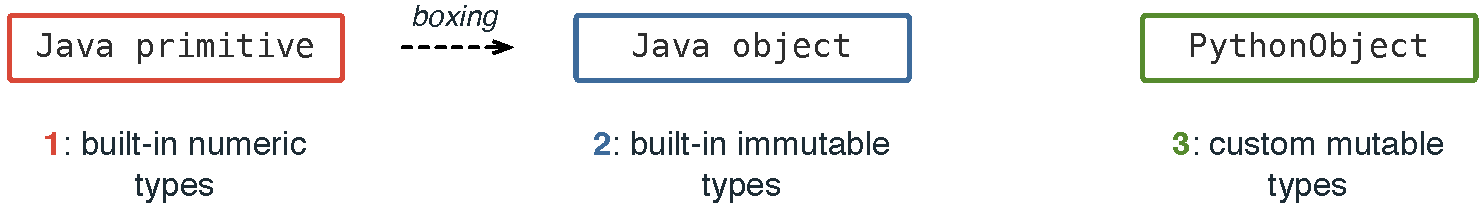
\includegraphics[scale=.6]{figures/ch5-three-data-representations}
\caption{Three data representations for Python objects}
\label{fig:ch5-three-data-representations}
\end{figure}

ZipPy internally uses multiple data representations to model Python objects.
Figure~\ref{fig:ch5-three-data-representations} illustrates this design scheme:

\begin{enumerate}

\item \textbf{Built-in numeric types}
ZipPy as explained in Chapter~\ref{sec:ch3-design-and-implementation} models some built-in numeric types, like \texttt{bool}, \texttt{int} and \texttt{float}, using Java primitives.
This approach helps to achieve Java level performance for arithmetic operations in ZipPy.
We refer types that has a Java primitive representation as \emph{unboxable}.
Each \emph{unboxable} numeric type in ZipPy has a corresponding \emph{boxed} representation using Java objects as a fallback.
As shown in the Figure, a boxing operation will convert an instance of unboxable type, e.g., \texttt{int}, from its Java primitive representation to the boxed one.

\item \textbf{Built-in immutable types}
Similar to Jython, we implement Python built-in types including numeric types as regular Java classes.
In this way we map Python's built-in type hierarchy onto a Java class based type hierarchy.
Unlike custom types, all built-in types in Python are immutable meaning that user program cannot modify the attributes of an instance of a built-in type.
We take advantage of this immutability by modeling Python built-in types directly using Java classes on the JVM.

\item \textbf{Custom mutable types}
All custom or user defined types in Python are mutable.
That includes Python modules, custom type definitions written in Python and instances of custom classes.
We model them using still a regular Java object, an instance of \texttt{PythonObject} in ZipPy, to circumvent the performance overhead incurred by using a hash map.
ZipPy maps Python attribute accesses to field accesses on the \texttt{PythonObject} object.
We support attribute mutation by maintaining an object layout table for each Python object.
The object layout table keeps track of the memory offset for each attribute that is currently alive on the object.
We will discuss how we support attribute mutations on Python types in more detail in Section~\ref{sec:ch5-custom-mutable-types}.

\end{enumerate}

Although we model Python objects using different physical data representations, our approach preserve the semantics that every data in Python is an object.
ZipPy support object like operations on each of the data representations described above.
What differs our approach to the existing ones is that we do not treat all Python data types in the same way.
We try to pick the most efficient construct offered by the JVM that is suitable for implementing particular types in Python.
To be more specific, modeling Python numbers as Java primitives enables the best arithmetics performance achievable on the JVM.
Using Java object to model Python object brings the potential for ZipPy to close the performance gap of object operations between Python and Java.

\subsection{Attribute Resolutions}

Each object in Python is a collection of key value pairs.
Each key value pair is an attribute of the object with the key being the symbol of the attribute.
The value of an attribute is essentially another Python object.
Like other dynamic languages, Python allows programmers to reference, add or delete attributes on an object.
Attribute referencing follows a rule referred as method resolution order in Python.
Upon the creation of a custom type or class in Python, the interpreter calculates a linearized list of types for the newly created type.
Each type in the list is a super type of the new type.
The method resolution order of the new type refers to the order its super types appear in the linearized list.
Given the method resolution order, an attribute resolution on a Python object follows the following steps:

\begin{enumerate}

\item Lookup the attribute from the object itself.
If it does not exist on the object, continue with the next step.

\item Obtaining the class object of the original object through the \texttt{\_\_class\_\_} attribute of the object.
Lookup the attribute from the class object.
If failed, continue with the next step.

\item Obtaining the bases of the object's class through the \texttt{\_\_bases\_\_} attribute of the class object.
Lookup the bases types in the method resolution order until the attribute is found.
Otherwise, if the interpreter fail to resolve the attribute in the end, it throws an \texttt{AttributeError}.

\end{enumerate}

\begin{figure}
\centering
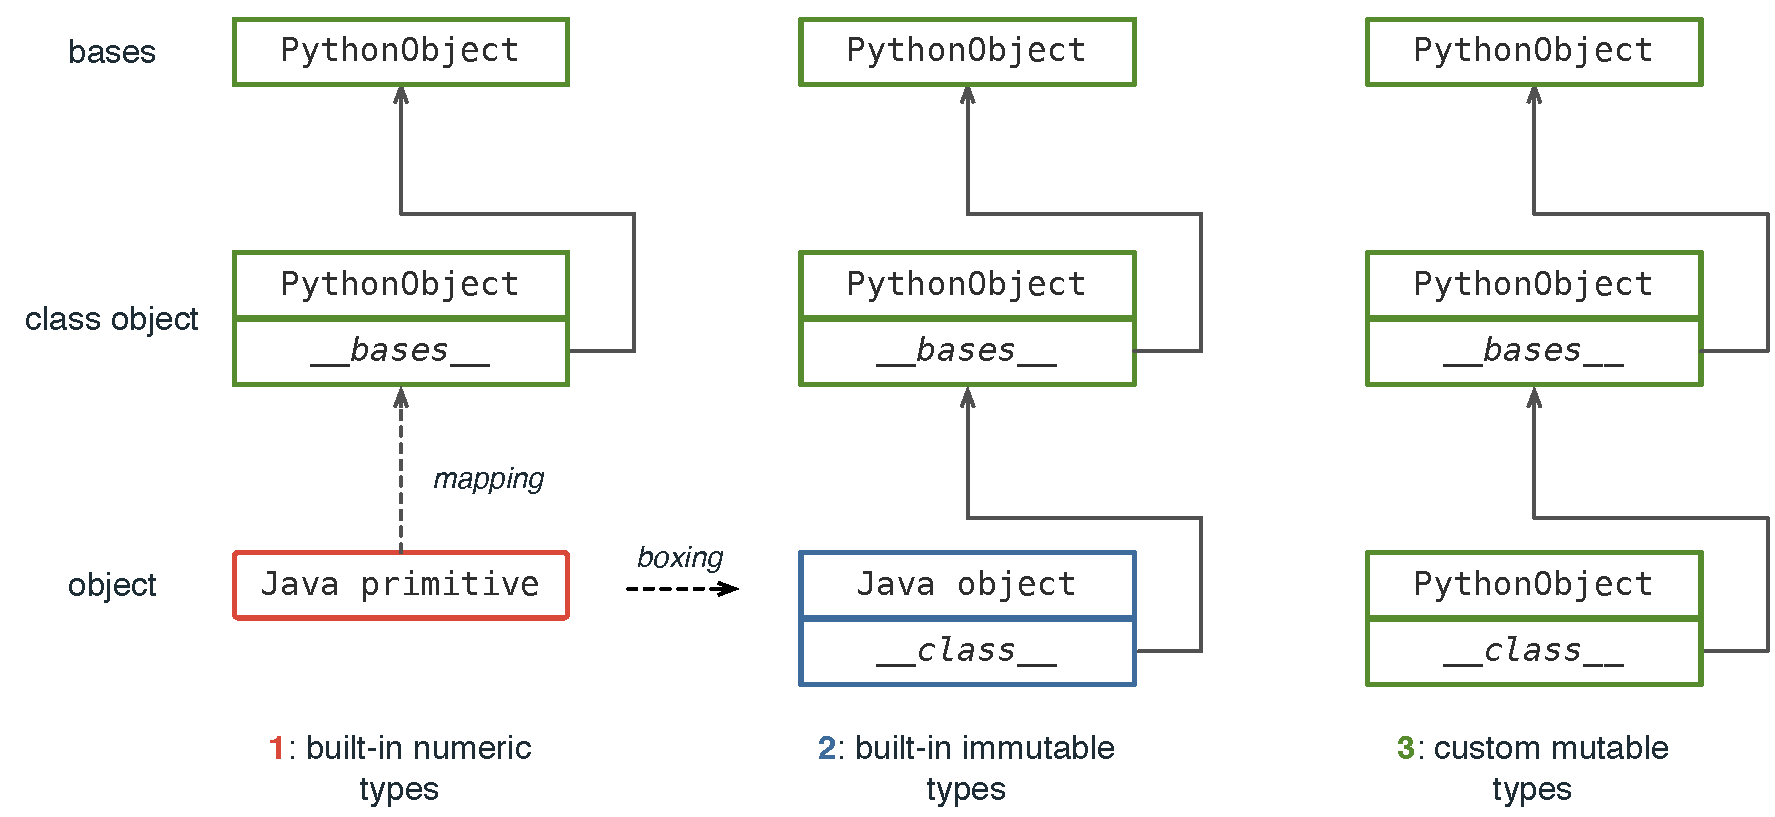
\includegraphics[scale=.54]{figures/ch5-attribute-resolutions}
\caption{Attribute resolution for different data representations}
\label{fig:ch5-attribute-resolutions}
\end{figure}

Since ZipPy uses multiple data representations to model Python objects, we also need to implement the above mentioned attribute resolution differently for each representation.
Figure~\ref{fig:ch5-attribute-resolutions} illustrates this process for the three different data representations used in ZipPy.
For simplicity, we model all class objects using a mutable \texttt{PythonObject}.
Each \texttt{PythonObject} stores the reference to the next node in the lookup chain as a dedicated field (\texttt{\_\_class\_\_} and \texttt{\_\_bases\_\_}).
This choice makes the type hierarchy of mutable objects consistent, since every node on the lookup chain is a \texttt{PythonObject}.
Similarly, built-in types modeled using immutable java objects connect to the rest of the lookup chain also use a reference stored in a dedicated field.
For unboxed built-in types, we uses a preprocessed mapping table to associate the Java class of the primitive type to the class object representing its Python type.
For instance, we model a Python integer, which is an instance of the Python \texttt{int} class, using a Java primitive \texttt{int}.
However, we model the Python \texttt{int} class object itself, which is an instance of the class \texttt{type}, using a mutable Java object.
The mapping table maps the Java class of primitive \texttt{int} to the Python \texttt{int} class object, and therefore completes the entire lookup chain for unboxed built-in types.

\subsection{Modeling Custom Mutable Types}
\label{sec:ch5-custom-mutable-types}

\begin{figure}
\centering
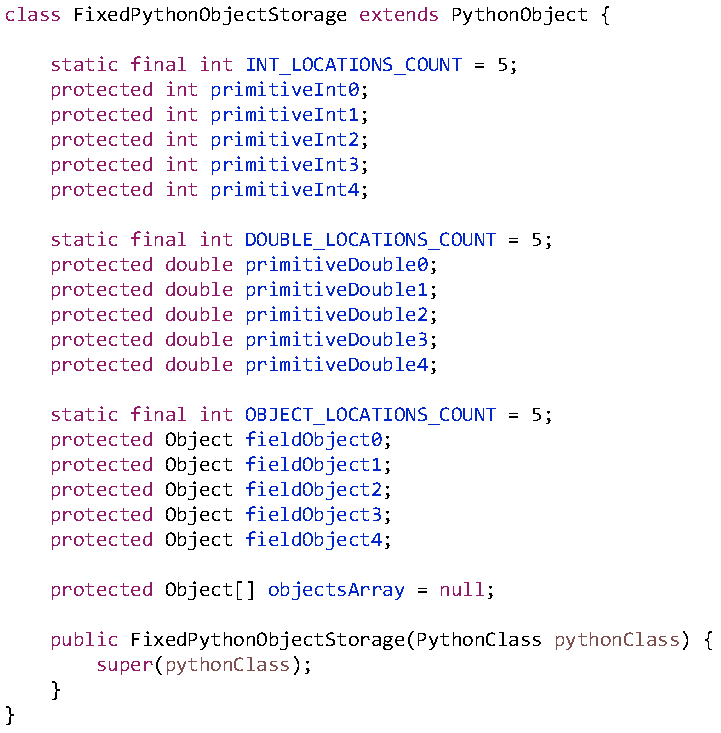
\includegraphics[scale=1.]{figures/ch5-fixed-python-object-code}
\caption{The implementation of \texttt{PythonObject}}
\label{ch5-fixed-python-object-code}
\end{figure}

\begin{figure}
\centering
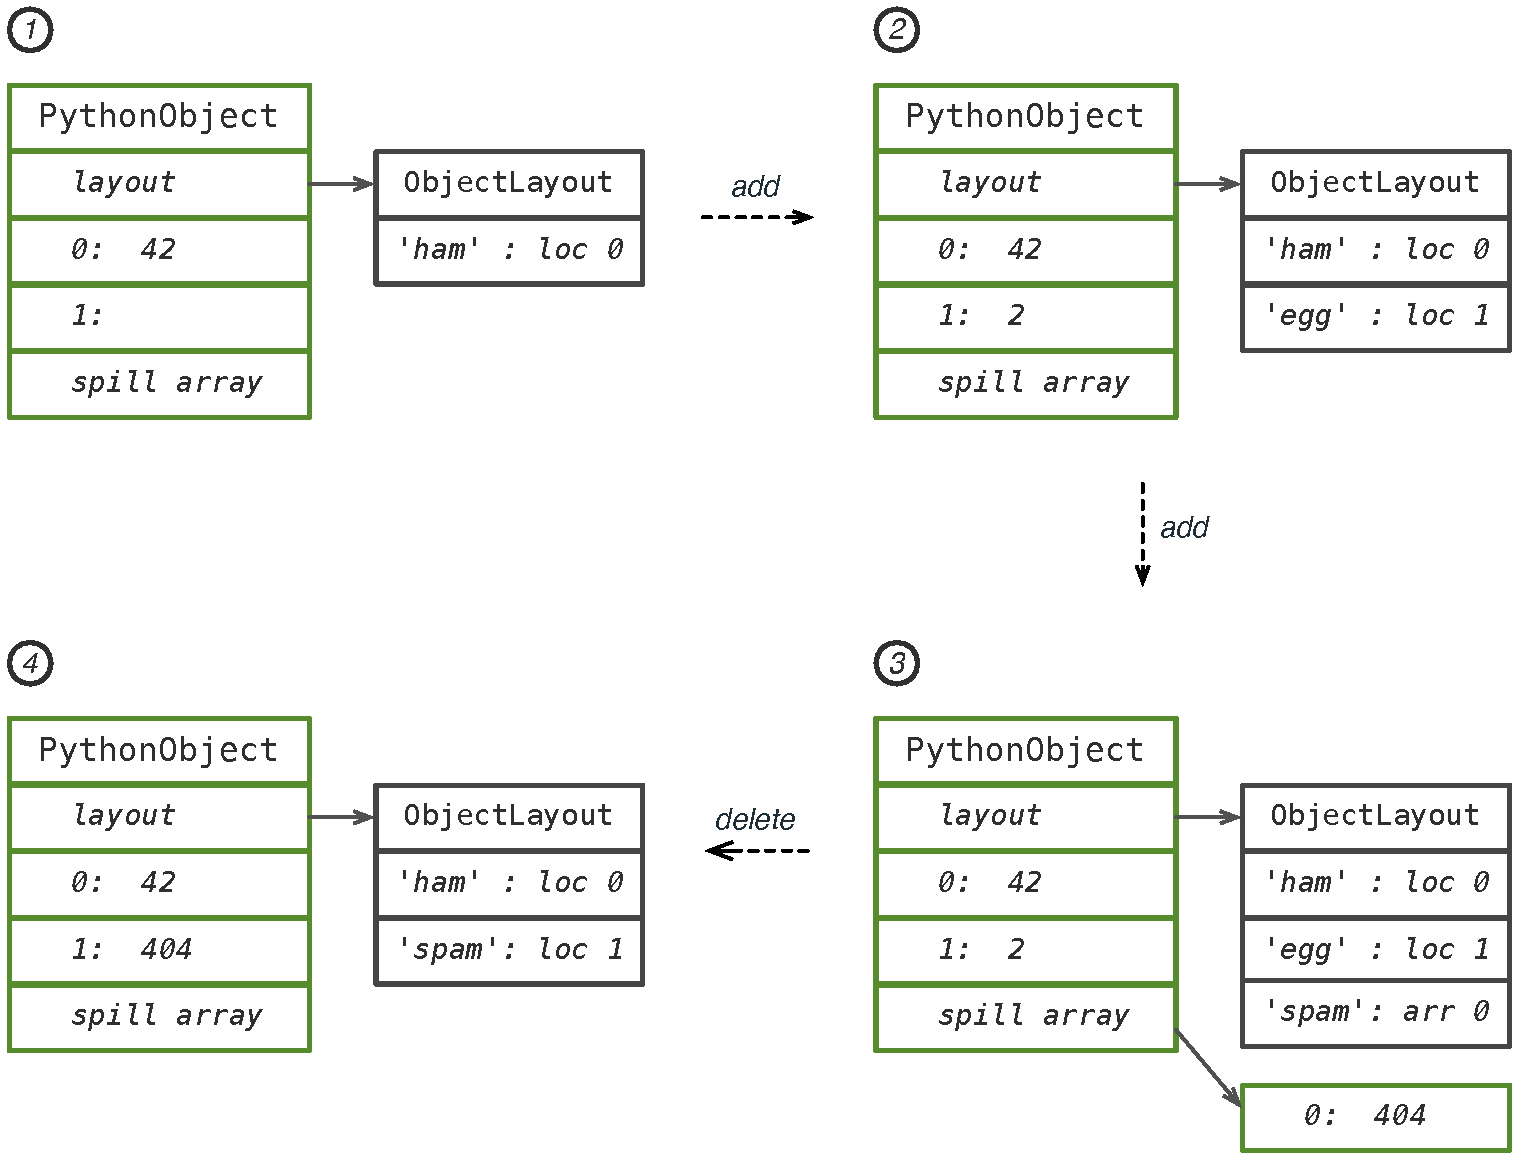
\includegraphics[scale=.6]{figures/ch5-mutable-object-layout-change}
\caption{Mutable object layout}
\label{ch5-mutable-object-layout-change}
\end{figure}

Python allows programmers to add, modify or delete attributes on an object during the execution of the program.
On the other hand, a Java object is fixed.
You can modify the value of a field, but cannot resize or change the layout of an object.
We support this dynamic feature of Python by implementing each Python object using a combination of a fixed \texttt{PythonObject} and a resizable object layout.

Figure~\ref{ch5-fixed-python-object-code} shows an implementation of \texttt{PythonObject} in ZipPy.
Each \texttt{PythonObject} has a fixed number of fields of both primitive and reference types to accommodate its attributes.
Each field on the objec is a \emph{location}.
The object stores each of its attribute on a dedicated \emph{location}.
ZipPy tries to store an unboxed attribute in an unboxed location to avoid the overhead of boxing.
For instance, it tries to store a Java \texttt{int} in an \texttt{int} field when possible.
If all \texttt{int} fields are taken, it tries to stores the attribute in an \emph{boxed} location or an object field.
If no in-object location is available anymore (taken by other attributes), ZipPy will spill the incoming attribute the additional object array (field \texttt{objectArray} in Figure~\ref{ch5-fixed-python-object-code}).
The additional object array gives the fixed \texttt{PythonObject} the ability to store more attributes than its own capacity by paying the price of another level of direction and possibly auto-boxing.

An object layout attached to a \texttt{PythonObject} keeps track of the list of attributes stored on the object as well as the location of each attribute.
It is essentially a table that maps the symbol of an attribute to its location.
The table records modifications made dynamically to the attributes of the object.
Figure~\ref{ch5-mutable-object-layout-change} illustrates how this process works by using a hyperthetical Python object.
The layout of the shown object goes through the following stages:

\begin{enumerate}

\item The object initially has one attribute \textsf{ham} stored in location $0$ with the value $42$.

\item After adding the attribute \textsf{egg}, the object now has both \textsf{ham} and \textsf{egg} stored in location $0$ and $1$ respectively.

\item Since both in-object locations are taken, the object stores the new attribute \textsf{spam} in the spill array at the index $0$.
The rest of the layout remain unchanged.

\item The deletion of \textsf{egg} frees location $1$ on the object.
The object reassigns the newly available in-object location to \textsf{spam} to make sure that location assignments are optimal.
It also update the layout table to reflect the new changes.

\end{enumerate}

We simplified the structure of the Python object shown in Figure~\ref{ch5-mutable-object-layout-change} for brevity.
The actual algorithm for a layout update is more complicated.
Adding or deleting an attribute triggers a layout update.
The update tries to stores as many unboxed attributes in an unboxed location as possible.
The spill array allocation is lazy that we only allocate the array when necessary.
During the layout update, ZipPy calculates the size of the addtional spill array needed to accommodate all the attributes.
If it requires a spill array, we conservatively allocate an array that is just enough to store all the attributes.

The type of an attribute can change at runtime.
Type change also triggers a layout update.


\subsection{Inline Caching for Attribute Accesses}

\section{Call Site Modeling}

Calls are common in Python programs.
In general you can call any \emph{callable} object in Python.
Making a call in different contexts has different semantics allowing the caller to pass arguments to the callee in different ways.

\subsection{Call Sites Structures in Python}
\label{sec:ch5-structure-of-call-sites}

\begin{figure}
\centering
\subfigure[Simple call site]{
	
\includegraphics[scale=.9]{figures/ch5-call-site-simple-code}
	\label{fig:ch5-call-site-simple-code}
}
\subfigure[Attribute call site]{
	
\includegraphics[scale=.9]{figures/ch5-call-site-attribute-code}
	\label{fig:ch5-call-site-attribute-code}
}
\caption{Basic syntax of calls in Python}
\label{fig:ch5-call-site-synteax-code}
\end{figure}

Figure~\ref{fig:ch5-call-site-simple-code} shows the syntax of a simple call in Python.
It is simple enough for us to explain the basic steps of making a call in Python without getting into more complicated details.
The execution of the call shown in the Figure involves the following steps.
As the first step, the program needs to look up the symbol \texttt{foo} from the current scope or its enclosing scope with respect to Python's scoping rules.
After resolving the symbol \texttt{foo}, the program then checks the type of the resolved object to determine the eligibility of such call.
Lastly, the actual call takes place using a calling convention that matches the type of the callee object.
The Python interpreter uses different calling convention or passes the arguments to the callee in a different way depending on the actual type of the callee.
For instance, if the callee is a Python class object, the interpreter creates an empty Python object and passes it to the callee as the first argument.

The call site shown in Figure~\ref{fig:ch5-call-site-simple-code} is in its simplest form.
We refer it as a \emph{simple call site}.
The callee resolution for the call shown in Figure~\ref{fig:ch5-call-site-attribute-code} involves an attribute referencing on the Python object \texttt{p}.
We refer this type of call sites as \emph{attribute call sites}, since the actual callee is an attribute of the primary object like \texttt{p} in the Figure.
The primary object, however, can be any namespace backed by a Python object such as a regular object, a class object or a module.
Looking back at the simple call site as shown in Figure~\ref{fig:ch5-call-site-simple-code},
it is worth noting that the callee resolution might involve an attributing referencing as well depending on the type of the scope in which the call takes place.
For example, if program resolves \texttt{foo} as a global variable, the look up of \texttt{foo} includes an implicit attribute referencing on the current Python module.
Similarly, in a class scope, a simple call to an existing class attribute also involves an implicit attribute look up on the enclosing class object.
% say something about motivates the structure of the AST
The same syntax implies different semantics and ways to make the actual call at runtime.
To capture this variation, we decompose a call site in Python into multiple components and assemble them in different ways to serve different variations.
This way allows us to apply specializations on each component separately to accelerate calls in Python programs.

\subsubsection{The AST of Call Sites}

\begin{figure}
\centering
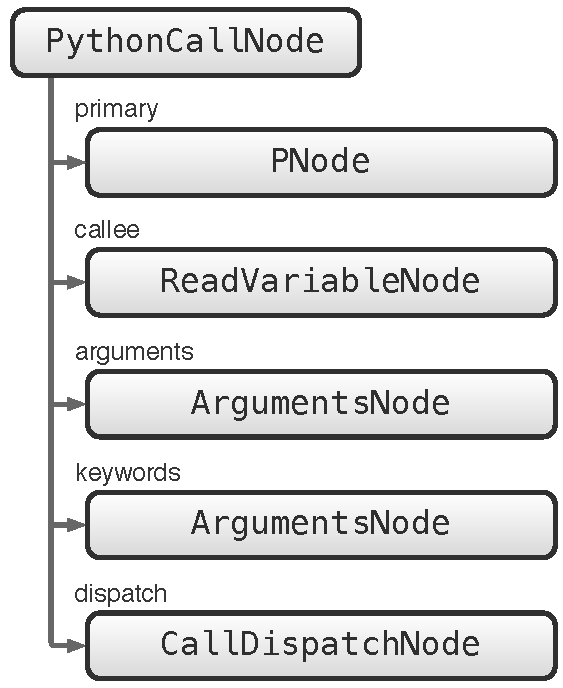
\includegraphics[scale=.5]{figures/ch5-python-call-node-basic}
\caption{The structure of a \texttt{PythonCallNode}}
\label{fig:ch5-python-call-node-basic}
\end{figure}

Figure~\ref{fig:ch5-python-call-node-basic} illustrates the basic structure of a call node in ZipPy.
A \texttt{PythonCallNode} employees five child nodes representing five components of the call site.
Each child node can further expand into its own sub tree depending on the complexity of the component.
A call node performs a Python call in-coorperating its child nodes in the following steps:

\begin{enumerate}

\item The primary node evaluates the primary object of the call.
If the primary component is missing, the primary node returns the constant Python \texttt{None} object.

\item The callee node resolves the actual callee object using the previously resolved primary object if necessary.
If the callee resolution does not involve an attribute referencing, it ignores the primary object.

\item The arguments node evaluates all the arguments, and returns them to the call node as a Java array.

\item The keywords node evaluates all the keyword arguments, and returns them to the call node in an Java array.

\item The \texttt{PythonCallNode} passes the evaluated primary object, callee, arguments array and keyword arguments array to the dispatch node.
The dispatch node performs the actual call using an inline caching inspired dispatch chain scheme~\cite{Deutsch1984, holzle1991}, and passes all the arguments to the AST of the callee.
We will explain the call dispatch nodes in more detail in Section~\ref{sec:ch5-call-site-caching-and-inlining}.

\end{enumerate}

Note that some components like the primary or keyword arguments are not always present.
In case that an optional component is missing, we still model it as a dummy node that returns a \texttt{None} or an empty Java array to make it consistent for all call nodes.
The \texttt{PythonCallNode} organizes different components of the call site and handles transformations like type specialization and de-optimization at runtime.

\subsection{Call Node Specializations}

Similar to the type specializations of arithmetics as we discussed in Chapter~\ref{chp:ch3-zippy}, ZipPy applies specializations to call nodes against the type of the callee through node rewriting.
The interpreter initially constructs a call node using the uninitialized version (\texttt{UninitCallNode} in Figure~\ref{fig:ch5-call-node-specialization-simple}).
Upon the first execution of the call, the uninitialized call node uses a slow path to resolve the primary object and callee.
At the same time, it rewrites itself to a derivative version that is tailored to the resolved primary and callee.
Not only that the call node specializes itself, it also applies type specializations to its child nodes during the rewriting process.
In this Section, we explain how ZipPy applies call node specializations for different call sites and callee types.

\subsubsection{Specialization for Simple Call Sites}

\begin{figure}
\centering
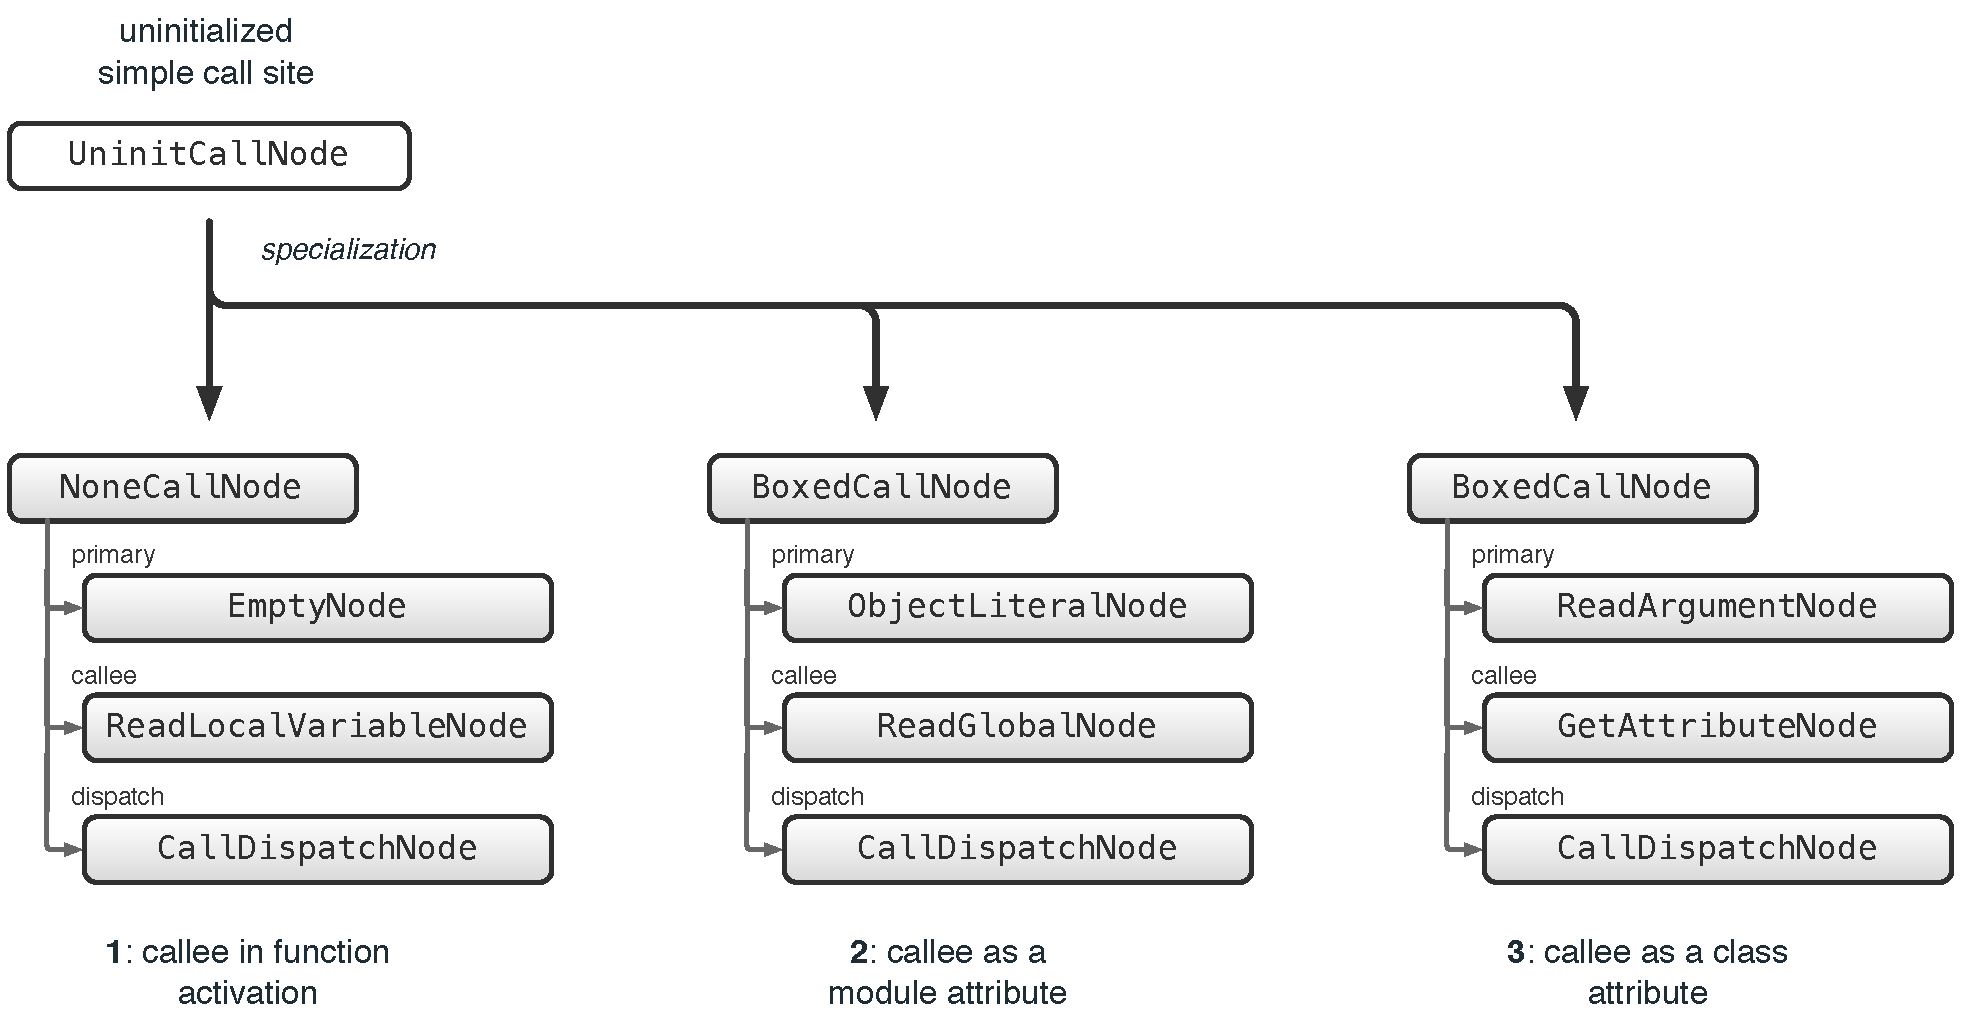
\includegraphics[scale=.5]{figures/ch5-call-node-specialization-simple}
\caption{Call node specializations for a simple call site}
\label{fig:ch5-call-node-specialization-simple}
\end{figure}

As explained in Section~\ref{sec:ch5-structure-of-call-sites}, the callee resolution of a simple call site (Figure~\ref{fig:ch5-call-site-simple-code}) depends on the type of the namespace to which the callee belongs.
Therefore, the specialization of a simple call site needs to cover different resolution cases.
Figure~\ref{fig:ch5-call-node-specialization-simple} illustrates various call node transformations of a simple call site.
The description of the three different specialization cases shown in the Figure is as follows:

\begin{enumerate}

\item \textbf{Callee in function activation}
The call takes place in a function scope.
The resolved callee is a variable of the function's lexical scope or its enclosing scope.
The primary object does not exist or is \texttt{None} in this case.
Therefore, the primary node is an \texttt{EmptyNode} that returns an \texttt{None}.
The callee nodes retrieve the callee object from the function's activation or the frame object as discussed in Chapter~\ref{sec:ch4-frame-and-control}.
Although type specialization is also applicable to the \texttt{ReadLocalVariableNode}, given that the callee is guarantee to be a boxed object, type specialization in this case has limited benefit.
However, Truffle is still able to optimize frame accesses by eliminating heap allocation of the frame object when applicable.

\item \textbf{Callee as a module attribute}
The resolved callee is an attribute of a module, e.g., the global scope of the current module or the built-in module.
The retrieval of the callee in this case involves an implicit attribute referencing on the primary module object.
Since the primary object is boxed, ZipPy specializes the call node to a \texttt{BoxedCallNode}.
The primary node is a wrapper node that holds a reference to the current module object.
The callee node reads the callee attribute from the module object returned by the primary node.
The \texttt{ReadGlobalNode} accesses the built-in module if it failed to resolve it from the global scope module.
Upon a successful resolution of the callee object, the \texttt{ReadGlobalNode} caches the actual primary object.
For instance, if the resolved callee object is an attribute of the built-in object, the node caches the built-in object instead of the current module.
Caching speedups subsequent attribute accesses by accessing the cached object directly as long as the attributes of the object remain unchanged.

\item \textbf{Callee as a class attribute}
The call takes place in a class scope.
The resolved callee is an existing class attribute of the enclosing scope.
Class definition works as a special function in Python.
The evaluation of the class definition statement is essentially a call to the special function.
The interpreter passes an empty class object as the first argument to the function, and the class definition function populates the class object with attributes like functions.
The call to the class definition function returns the created class object containing attributes specified by in the class definition.
To access an existing attribute of the defining class, we need to first retrieve the defining class object.
The \texttt{ReadArgumentNode} does so by reading the argument array passed by the caller of the class definition.
the callee node then reads the callee attribute from the primary class object.
The \texttt{GetAttributeNode} also enjoys type specialization and caching on its own, which we will discuss more in Section~\ref{sec:ch5-object-module}.

\end{enumerate}

The call node specializations illustrated in Figure~\ref{fig:ch5-call-node-specialization-simple} are based on the resolution of the primary object and callee.
We simplified the Figure to not show the arguments node and the keyword arguments node, since their specialization are orthogonal callee resolutions.

\subsubsection{Specialization for Attribute Call Sites}

\begin{figure}
\centering
\subfigure[Boxed primary]{
	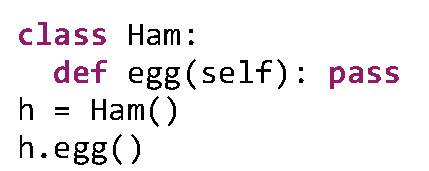
\includegraphics[scale=.7]{figures/ch5-attribute-call-site-boxed-code}
	\label{fig:ch5-attribute-call-site-boxed-code}
}
\subfigure[Unboxed primary]{
	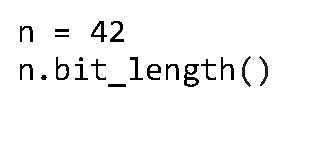
\includegraphics[scale=.7]{figures/ch5-attribute-call-site-unboxed-code}
	\label{fig:ch5-attribute-call-site-unboxed-code}
}
\caption{Attribute call sites with different primary object representations}
\label{fig:ch5-attribute-call-site-boxed-unboxed-code}
\end{figure}

In Chapter~\ref{sec:ch3-design-and-implementation} we discussed that ZipPy models Python objects using multiple data representations to make arithmetics and data accesses more efficient.
Since the physical data representation of Python objects differs in ZipPy, attribute lookups on objects backed by different representations are also different.
Figure~\ref{fig:ch5-attribute-call-site-boxed-unboxed-code} shows two attribute call sites.
The primary object of the left one, \texttt{h}, is a user custom Python object (Figure~\ref{fig:ch5-attribute-call-site-boxed-code}).
The primary object \texttt{n} in the one shown in Figure~\ref{fig:ch5-attribute-call-site-unboxed-code} is a built-in integer.
In ZipPy, we model custom objects using a boxed Java object, and map an attribute access to the Python object to a field access on the Java object.
On the other hand, ZipPy represents Python integers and some other built-in data types as Java primitives.
% probably did not explain it very clearly....
Therefore, attribute lookup on those built-in types involves a mapping that associates the instance of the type to the meta class object of the type containing the target attribute.

\begin{figure}
\centering
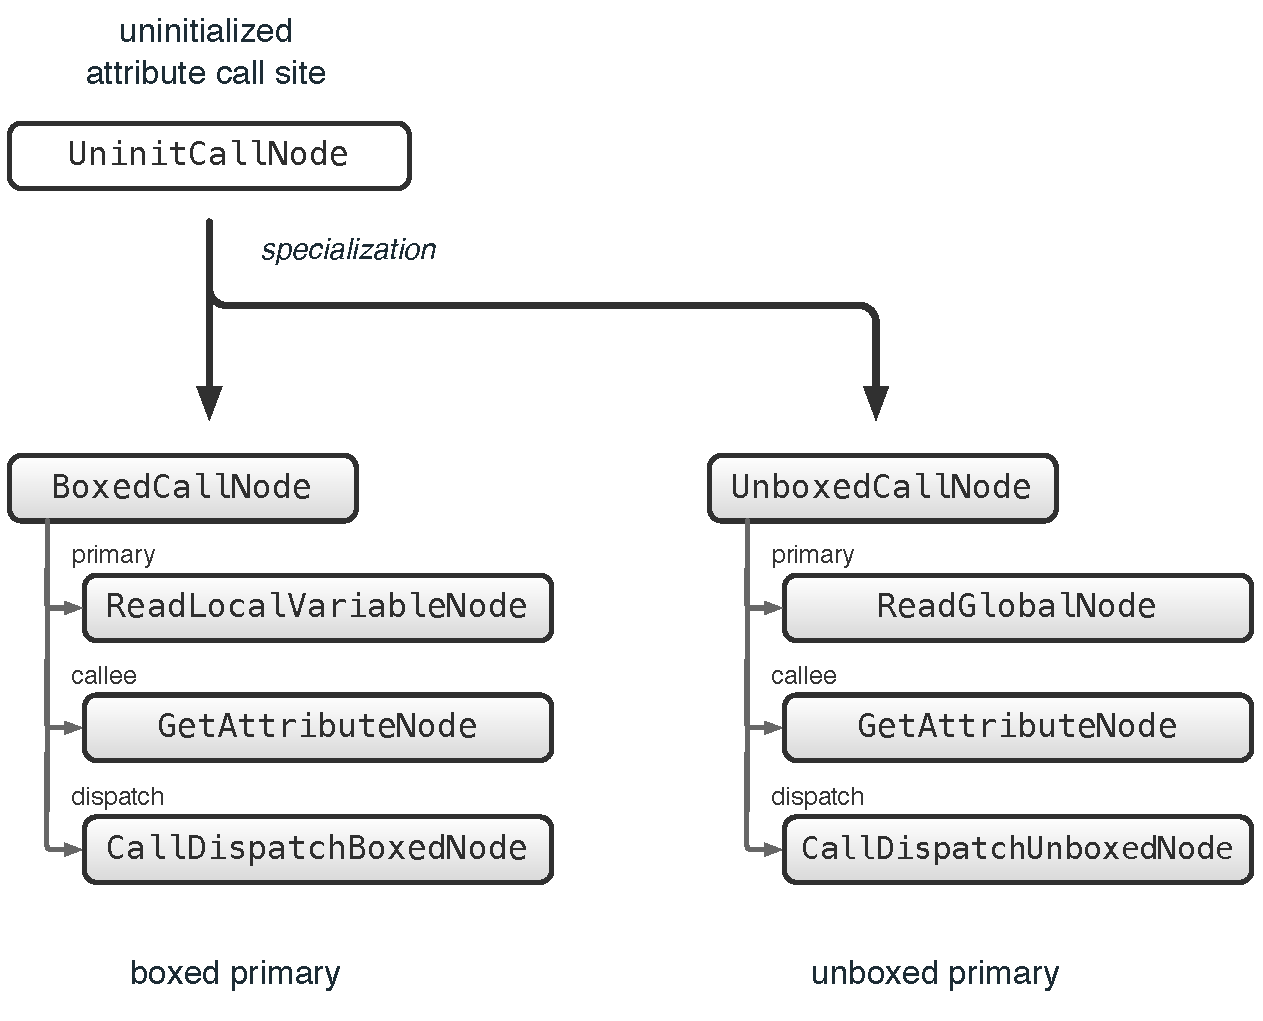
\includegraphics[scale=.5]{figures/ch5-call-node-specialization-attribute}
\caption{Call node specializations for an attribute call site}
\label{fig:ch5-call-node-specialization-attribute}
\end{figure}


% the specializations shown above covers the majority of calls in Python.
% However, they are not meant to be comprehensive. there are corner cases that we do not cover in this thesis due to space limitations.
% call node specialization captures the fast path of callee resolution.....
% the next chapter will talk about how we further optimize calls in Python.

\subsection{Call Site Caching and Inlining}
\label{sec:ch5-call-site-caching-and-inlining}

\subsection{Inline Caching Based Call Dispatching}

\subsection{Call Inlining in Truffle}
